\documentclass[conference]{IEEEtran}
\IEEEoverridecommandlockouts%
% The preceding line only needs to identify funding in the first footnote. If that is unnecessary, please comment on it.
\usepackage{cite}
\usepackage{amsmath,amssymb,amsfonts}
\usepackage{algorithmic}
\usepackage{graphicx}
\usepackage{textcomp}
\usepackage{xcolor}
\usepackage{hyperref}
\usepackage{caption}
\usepackage{comment}
\usepackage{colortbl}
\usepackage{booktabs}
\usepackage{tabularx}
\usepackage[most]{tcolorbox}
\usepackage{pdfpages}

\newenvironment{bgquote} {\begin{tcolorbox}[ enhanced, breakable=true, colback=blue!5, colframe=white, boxrule=0pt, left=1em, right=1em, top=0.5em, bottom=0.5em, boxsep=0pt, width=\linewidth, before skip=0.5em, after skip=0.5em ]} {\end{tcolorbox}}

\def\BibTeX{{\rm B\kern-.05em{\sc i\kern-.025em b}\kern-.08em
    T\kern-.1667em\lower.7ex\hbox{E}\kern-.125emX}}

\begin{document}

\title{Deep Learning-Based Super-Resolution of SAR Imagery Using UNet and ESRGAN\\
%{\footnotesize \textsuperscript{*}Note: Subtitles should not be used}
}

\author{\IEEEauthorblockN{Suraj Karki}
\IEEEauthorblockA{\textit{Department of Engineering Science }\\
\textit{University West}\\
Trollhättan, Sweden \\
suraj.karki@student.hv.se}
\and
\IEEEauthorblockN{Shumail Alam Khan}
\IEEEauthorblockA{\textit{Department of Engineering Science} \\
\textit{University West}\\
Trollhättan, Sweden \\
shumail.alam@student.hv.se}
}

\maketitle

\thispagestyle{plain}
\pagestyle{plain}


\begin{IEEEkeywords}
    SAR image super-resolution, deep learning, UNet, ESRGAN, speckle noise reduction, remote sensing, image reconstruction, generative adversarial networks, synthetic aperture radar, image enhancement
\end{IEEEkeywords}
\begin{abstract}
    Synthetic Aperture Radar (SAR) imagery plays a critical role in remote sensing applications due to its ability to operate under all-weather and day–night conditions. However, SAR images are inherently affected by speckle noise and limited spatial resolution, which restrict their effectiveness for fine-grained analysis. This study presents a deep learning-based framework for SAR image super-resolution using two architectures: UNet and ESRGAN. The objective is to reconstruct high-resolution (HR) SAR images from low-resolution (LR) inputs while preserving structural integrity and reducing noise-induced artefacts. A paired dataset derived from the JERS-1 SAR Global Rain Forest Mapping Project is used, with synthetic degradation applied to generate LR–HR training pairs. The models are trained and evaluated using both quantitative metrics, including Peak Signal-to-Noise Ratio (PSNR) and Structural Similarity Index (SSIM), and qualitative visual assessment. Experimental results show that UNet provides stable reconstruction with consistent structural preservation, while ESRGAN achieves superior performance in terms of both PSNR and SSIM, along with improved visual fidelity and sharper texture reconstruction. The study further highlights the trade-off between pixel-wise accuracy and perceptual quality in super-resolution tasks. Despite limited computational resources and reduced training duration, the proposed ESRGAN-based approach demonstrates strong potential for SAR image enhancement. The findings suggest that adversarial learning combined with appropriate preprocessing and augmentation strategies significantly improves SAR image reconstruction quality, offering a promising direction for future remote sensing applications
\end{abstract}

\section{Admin Part} 
The source code for this study can be found at~\cite{github_repo}.  

\subsection{Impact of EU AI Regulation on This Project}

The EU AI Act\cite{eu_ai_act_2024} introduces a risk-based framework governing the development and deployment of AI systems within the European Union. In the context of this project, which focuses on SAR image super-resolution using UNet and ESRGAN, the system is primarily developed for research and academic purposes. As such, it would generally fall outside strict regulatory obligations during development, provided it is not deployed in real-world decision-making scenarios.

However, if the proposed system were to be applied in operational domains such as remote sensing, environmental monitoring, or surveillance, it could fall under high-risk AI categories, particularly where decisions impact safety, security, or fundamental rights. In such cases, the regulation would require compliance with strict standards, including data governance, model transparency, robustness, and risk management.

From a design perspective, this project already aligns with several key principles of the regulation. The inclusion of quantitative metrics (PSNR, SSIM) alongside qualitative visual validation supports transparency and performance evaluation. Additionally, documenting limitations eg, potential artefacts introduced by UNet, helps address the risk of misleading outputs, which is critical when dealing with reconstructed SAR imagery.

Furthermore, the regulation emphasises human oversight, meaning that any deployment of this system should ensure that enhanced images are interpreted by domain experts rather than used for fully automated decision-making. This is particularly important in SAR applications, where incorrect reconstruction could lead to misinterpretation of terrain or objects.

\subsection{Contributions}
\begin{table*}[h!]
    \centering
    \renewcommand{\arraystretch}{1.3}
    \rowcolors{2}{white}{gray!10}
    \begin{tabularx}{\textwidth}{p{5cm}XX}
    \toprule
    \rowcolor{gray!20} \textbf{Task} & \textbf{Suraj Karki} & \textbf{Shumail Alam Khan} \\
    \midrule
    
    Data Collection & Responsible for acquiring and preparing the JERS-1 SAR dataset, including preprocessing and patch extraction pipeline setup. & Assisted in dataset validation and verification of preprocessing consistency across training, validation, and test splits. \\
    
    Article Selection and Literature Review & Contributed to identifying relevant SAR super-resolution and deep learning literature, focusing on ESRGAN and GAN-based methods. & Contributed to selection of UNet-related literature and jointly reviewed all selected papers for relevance and quality. \\
    
    Baseline Model Implementation & Implemented GAN-based baseline model (ESRGAN), including training pipeline, loss configuration, and adversarial setup. & Implemented UNet baseline model \\
    
    Further Iterations & Contributed to improvements in GAN training stability, loss balancing, including preprocessing refinements, augmentation tuning, and architectural adjustments. & Contributed to UNet improvements. \\
    
    Final Evaluation and Consolidation & Participated in quantitative evaluation (PSNR, SSIM) and qualitative assessment of both models. & Participated in result consolidation, comparison analysis, and interpretation of performance differences. \\
    
    Report Writing & Led drafting of sections related to ESRGAN, system engineering, and experimental results. & Led drafting of sections related to UNet, and requirements analysis. \\
    
    Review and Final Editing & Reviewed full report for clarity, structure, and final formatting corrections including latex formatting, github integration. & Reviewed full report for technical accuracy and consistency. \\
    
    \bottomrule
    \end{tabularx}
    \caption{Contribution breakdown of each author across the project.}
    \label{tab:author-contributions}
    \end{table*}

\subsection{Use of AI}
In this project, ChatGPT~\cite{chatgpt_2026} and Microsoft Copilot~\cite{microsoft_copilot} were used as assistive tools to support development and documentation. Their use included generating initial code snippets for data preprocessing, model architecture prototyping, and training loop implementation, as well as assisting in debugging and explaining relevant concepts in SAR imaging and deep learning methods. For report writing, these tools were used in a supportive role to improve structural organisation, refine technical phrasing, and enhance grammatical clarity, particularly in sections such as the abstract, and system descriptions. Some AI-assisted suggestions were used to improve readability in technically dense parts of the text, but all content was critically reviewed, rewritten where necessary, and validated against implemented experiments and results. Importantly, AI tools were not used to generate final conclusions, experimental outcomes, and core design decisions, and full responsibility for the technical correctness, interpretation, and validation belongs to the authors.

\section{Requirements and Data Analysis}
The objective of this project is to design and evaluate deep learning models for super-resolution of Synthetic Aperture Radar (SAR) images. Given a low-resolution (LR) SAR image, the system must reconstruct a super-resolution (SR) version that preserves structural details and minimises noise-induced artefacts.

SAR imagery presents unique challenges compared to optical images due to the presence of speckle noise, multiplicative noise characteristics, and lower signal-to-noise ratios. Therefore, the requirements extend beyond simple pixel reconstruction and must account for structural fidelity. The system should be evaluated using both quantitative metrics (e.g., PSNR, SSIM) and qualitative visual assessments to ensure that the reconstructed images are not only numerically accurate but also visually coherent. Additionally, the system should be designed to handle varying levels of noise and different types of SAR data, ensuring robustness across diverse scenarios.

The key functional requirements include:
1. The system must accept LR SAR images as input and produce corresponding super resolution SR images.
2. The reconstructed images must preserve edge structures, textures, and geometric features.
3. The system must minimise speckle amplification and artefacts.
4. The system should generalise across different SAR scenes.
5. The model should be computationally feasible for training on limited GPU/CPU resources.

Non functional requirements include:
1. Stability during training.
2. Reproducibility of results.
\subsection{Dataset}
The dataset used in this study is derived from the JERS-1 SAR Global Rain Forest Mapping Project \cite{chapman2015jers1}. This project produced the first high-resolution, wall-to-wall radar coverage of the Amazon Basin. The imagery was acquired by the Japanese Earth Resources Satellite-1 (JERS-1) using an L-band SAR sensor with a wavelength of 23.5 cm. This frequency enables effective penetration through cloud cover and strong interaction with vegetation structure, soil moisture, and flooded forest environments \cite{chapman2015jers1}.

The dataset comprises 66 GeoTIFF mosaic tiles at an approximate spatial resolution of 100 metres. These tiles represent two hydrological seasons, 32 tiles from the low-flood period (September to December 1995) and 34 tiles from the high-flood period (May to July 1996). Each mosaic tile is constructed from approximately 50 individual SAR scenes that have been radiometrically calibrated and mosaicked to ensure seamless regional coverage. The consistent acquisition geometry and standardised preprocessing pipeline result in stable and comparable backscatter characteristics across the entire dataset\cite{chapman2015jers1}.

For super-resolution modelling, image patches were extracted from the mosaics and organised into paired HR and synthetically downsampled LR samples. Prior to patch extraction, each image undergoes logarithmic transformation to compress the dynamic range of SAR intensities, followed by percentile-based normalisation using the 1st and 99th percentiles. This step ensures numerical stability and reduces the influence of extreme outliers while preserving relevant backscatter variations.

A structured data splitting strategy is employed, dividing the dataset into training, validation, and test subsets using fixed proportions. During training, multiple patches are sampled per image to improve data efficiency and increase variability.

To enhance model generalisation, several data augmentation techniques are applied to HR patches during training. These include random horizontal and vertical flipping, as well as random rotations by multiples of 90 degrees. In addition, synthetic speckle noise is introduced probabilistically to the LR patches using a multiplicative noise model. This augmentation reflects the physical characteristics of SAR imaging and enables the model to jointly learn despeckling and super-resolution.

LR patches are generated from HR counterparts using bicubic interpolation with anti-aliasing, ensuring a realistic degradation process. The resulting HR and LR patches are then converted into single-channel tensors suitable for deep learning models.

Visual inspection (Figure~\ref{fig:data_visualization}) shows that HR patches preserve fine-scale speckle patterns, vegetation texture, and hydrological structures, whereas LR patches exhibit smoothing effects and reduced variance due to downsampling. Histogram analysis further supports these observations. HR patches demonstrate a broader dynamic range with heavier-tailed intensity distributions, while LR patches exhibit narrower, more Gaussian-like distributions centred around similar mean values. This behaviour reflects the consistent radiometric calibration of the dataset and ensures a well-defined and physically meaningful relationship between LR and HR samples.

Overall, the dataset provides a robust and scientifically sound foundation for evaluating super-resolution techniques on large-scale, real-world SAR imagery.

\begin{figure*}[h!]
    \centering
    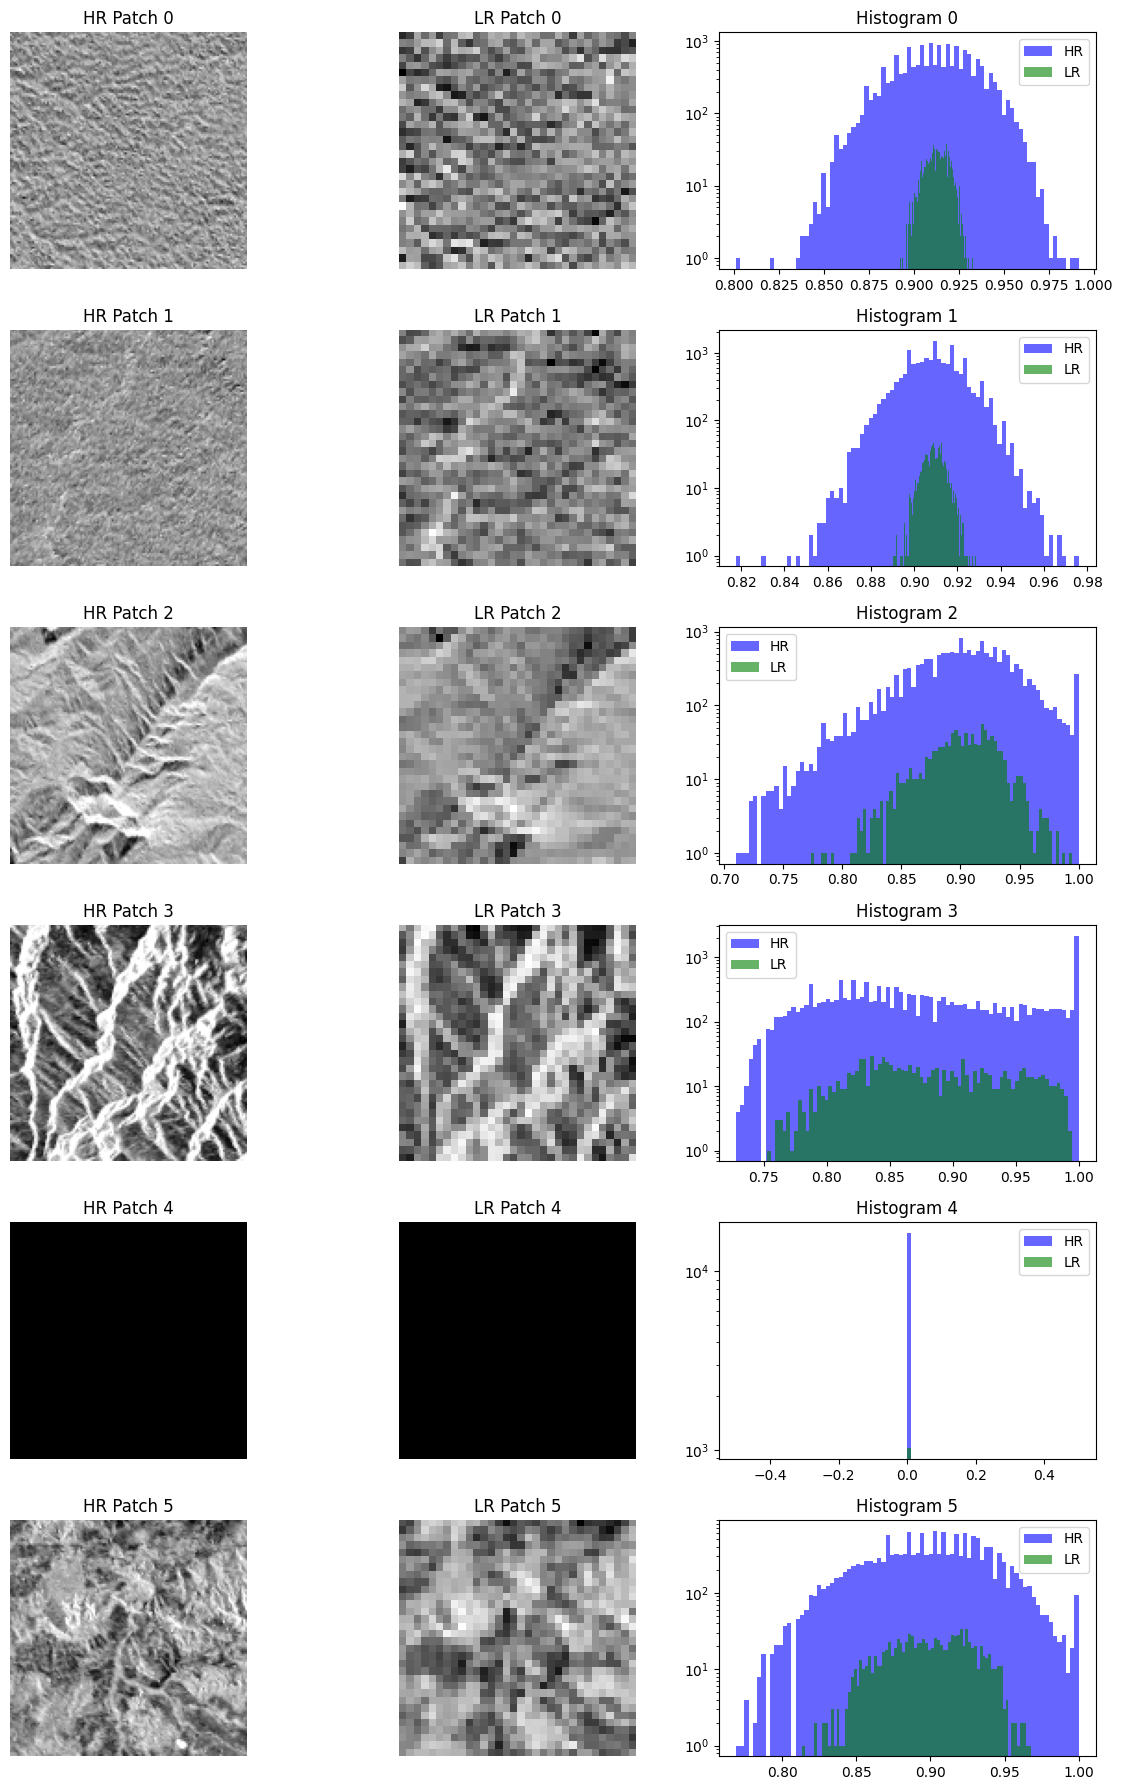
\includegraphics[width=\textwidth,height=0.7\textheight,keepaspectratio]{figures/data_visualization.png} 
    \caption{Examples of HR and LR image patches alongside their corresponding intensity histograms.}
    \label{fig:data_visualization}
\end{figure*}

\subsection{Requirements Analysis Based on Existing Research}

Existing research in Synthetic Aperture Radar (SAR) image processing highlights several challenges that directly influence the design of super-resolution models for real-world SAR data. SAR imagery is inherently affected by speckle noise, limited spatial resolution, and complex backscatter characteristics, which complicate the extraction of fine-grained structural and textural information\cite{curlander1991synthetic,debuysere2024synthesizing}. These challenges establish the need for robust enhancement techniques capable of improving image quality while preserving physically meaningful features.

A primary limitation in conventional SAR processing lies in the trade-off between spatial resolution and noise. High-resolution SAR acquisitions are costly and not always available, while lower-resolution products often exhibit smoothing effects that obscure important details. This creates a requirement for super-resolution methods that can reconstruct high-frequency details from degraded observations without introducing artificial artefacts\cite{yang2019deep}.

In addition, speckle noise remains a fundamental issue in SAR imaging due to its multiplicative nature. Traditional filtering techniques filters, reduce noise at the expense of spatial detail, often leading to loss of important structural information\cite{wei2025dynamical,electronics12132975}. Therefore, there is a strong requirement for approaches that can jointly perform despeckling and resolution enhancement while maintaining the statistical properties of SAR backscatter.

From a computational perspective, classical image reconstruction and enhancement methods are often not scalable to large datasets such as the JERS-1 mosaics used in this study. The increasing availability of SAR data demands efficient and automated pipelines capable of processing large volumes of imagery with minimal manual intervention\cite{zhu2017deep}. This introduces a requirement for learning-based models that can generalise across diverse scenes and operate efficiently during inference.

Recent advances in deep learning, have demonstrated strong potential in image super-resolution tasks\cite{Toosi2026S3ESRGAN},\cite{ye2024water},\cite{Song2022HAUnet}. However, most existing models are designed for natural images and do not explicitly account for the unique characteristics of SAR data, such as speckle noise distribution and radiometric behaviour. This gap creates a requirement for domain-specific model design and data preprocessing strategies tailored to SAR imagery\cite{Fracastoro2021Deep}.

Furthermore, the effectiveness of supervised learning approaches depends on the availability of high-quality training data. In SAR applications, true high-resolution ground truth is often unavailable. Consequently, synthetic degradation models are commonly used to generate low-resolution inputs from high-resolution data, requiring careful design to ensure physical realism\cite{electronics12132975}. This establishes a requirement for robust data preprocessing and augmentation strategies.

Based on these considerations, the following project-specific requirements are defined:

\begin{itemize}
    \item Effective super-resolution capability, reconstructing high-resolution SAR images from downsampled inputs while preserving structural and textural details.
    \item Integrated despeckling, reducing multiplicative speckle noise without oversmoothing or loss of important features.
    \item Preservation of radiometric consistency, ensuring that reconstructed images maintain physically meaningful backscatter characteristics.
    \item Computational efficiency and scalability, enabling processing of large-scale SAR datasets such as JERS-1 mosaics.
    \item Robust data preprocessing and augmentation, including realistic downsampling and noise modelling to support supervised learning.
    \item Generalisation across diverse scenes, ensuring stable performance across different land-cover types and hydrological conditions.
\end{itemize}

These requirements directly guide the design and implementation of the proposed deep learning framework, which leverages paired HR--LR SAR data and augmentation strategies to learn a mapping that enhances spatial resolution while simultaneously addressing speckle noise.

\subsection{System Specifications}

Based on the above identified requirements, a set of measurable and verifiable system specifications is derived to guide the development and evaluation of the proposed SAR super-resolution framework. These specifications translate qualitative objectives into quantitative criteria that can be assessed experimentally.

\subsubsection{Image Reconstruction Quality}

To ensure effective super resolution (SR), the reconstructed SR images must closely match the ground truth HR in both pixelwise accuracy and perceptual structure.

\begin{itemize}
    \item Peak Signal-to-Noise Ratio (PSNR): The model shall achieve a PSNR of at least 25 dB on the test dataset.
    \item Structural Similarity Index (SSIM): The model shall achieve an SSIM of at least 0.75, ensuring preservation of structural information.
    \item Visual fidelity: Reconstructed images shall preserve fine-scale textures such as speckle patterns, vegetation structures, and other relevant features such as hydrological.
\end{itemize}

\subsubsection{Speckle Reduction Performance}

The model must effectively reduce multiplicative speckle noise while maintaining important spatial details.

\begin{itemize}
    \item Noise suppression: Variance of homogeneous regions in reconstructed images shall be reduced compared to LR inputs.
    \item Edge preservation: Structural edges shall remain sharp, avoiding over-smoothing effects typical of traditional filters.
    \item Statistical consistency: Output images shall retain SAR-specific intensity distributions (non-Gaussian, heavy-tailed behaviour).
\end{itemize}

\subsubsection{Radiometric Consistency}

To maintain physical interpretability, reconstructed outputs must preserve radiometric properties of SAR backscatter.

\begin{itemize}
    \item Intensity range preservation: Output values shall remain within the normalised range [0,1].
    \item Histogram similarity: The intensity distribution of reconstructed images shall closely match that of HR ground truth (evaluated using histogram comparison metrics).
\end{itemize}

\subsubsection{Computational Efficiency}

The system must be computationally feasible for large-scale datasets.

\begin{itemize}
    \item Inference time: The model shall process a single $128 \times 128$ patch in less than 50 ms on a GPU.
    \item Scalability: The system shall support batch processing of large datasets without significant degradation in performance.
    \item Memory efficiency: The model shall operate within standard GPU memory constraints (e.g. $\leq$ 8–12 GB VRAM).
\end{itemize}

\subsubsection{Data Processing and Augmentation}

The preprocessing and data generation pipeline must ensure robustness and generalisation.

\begin{itemize}
    \item Patch generation: Each training image shall generate multiple patches to increase dataset diversity.
    \item Data augmentation: Random flips, rotations, and noise injection shall be applied during training.
    \item Degradation model: LR images shall be generated using bicubic downsampling with a scaling factor of $\times4$, combined with optional speckle noise.
\end{itemize}

\subsubsection{Generalisation and Robustness}

The model must generalise across different SAR scenes and conditions.

\begin{itemize}
    \item Cross-scene performance: The model shall maintain consistent PSNR and SSIM across validation and test datasets.
    \item Stability: Training shall converge without mode collapse or instability.
\end{itemize}

\subsubsection{Training Stability and Convergence}

For reliable model development, stable training behaviour is required.

\begin{itemize}
    \item Convergence: Training loss shall stabilise within a 5-epoch window.
    \item Model selection: The best-performing model shall be selected based on validation PSNR.
\end{itemize}

\subsubsection{Summary of Specifications}

Table~\ref{tab:system-specifications} summarises the key system specifications.

\begin{table*}[ht!]
    \centering
    \renewcommand{\arraystretch}{1.3}
    \rowcolors{2}{white}{gray!10}
    \begin{tabularx}{\textwidth}{p{3cm}XXX}
    \toprule
    \rowcolor{gray!20} \textbf{Specification} & \textbf{Metric / Measure} & \textbf{Target Value} & \textbf{Description} \\
    \midrule
    
    Image Quality & PSNR & $\geq$ 25 dB & Measures pixel-wise reconstruction accuracy between SR output and HR ground truth. \\
    
    Structural Preservation & SSIM & $\geq$ 0.75 & Ensures preservation of structural and textural information in SAR images. \\
    
    Super-Resolution Scale & Upscaling Factor & $\times 4$ & LR images are upscaled by a factor of four to generate HR outputs. \\
    
    Speckle Reduction & Variance Reduction & Lower than LR input & Evaluates effectiveness of despeckling in homogeneous regions while preserving details. \\
    
    Radiometric Consistency & Intensity Range & [0, 1] & Ensures output values remain within normalised SAR backscatter range. \\
    
    Histogram Consistency & Distribution Similarity & High similarity to HR & Maintains SAR-specific intensity distribution after reconstruction. \\
    
    Computational Efficiency & Inference Time & $<$ 50 ms per patch & Time required to process a $128 \times 128$ patch on GPU.\\
    
    Memory Constraint & GPU Usage & $\leq$ 8--12 GB & Ensures compatibility with standard hardware resources. \\
    
    Data Processing & Patch Size & $128 \times 128$ & Size of extracted HR patches used for training and inference. \\
    
    Data Augmentation & Techniques & Flip, rotation, noise & Includes geometric transformations and speckle noise injection. \\
    
    Scalability & Dataset Handling & Large-scale support & Ability to process multiple SAR tiles efficiently. \\
    
    Model Stability & Training Behaviour & Stable convergence & Ensures no divergence or instability during training. \\
    
    \bottomrule
    \end{tabularx}
    \caption{System specifications derived from project requirements, defining measurable criteria for evaluating the performance, efficiency, and robustness of the proposed SAR super-resolution framework.}\label{tab:system-specifications}
\end{table*}

\section{System Engineering}
\subsection{System Overview}

Based on the derived specifications, a modular system architecture is designed for SAR image super-resolution and despeckling. The system follows a data-driven deep learning pipeline, where LR SAR images are transformed into SR outputs using either a UNet or ESRGAN-based model.

Figure~\ref{fig:system_architecture} illustrates the overall system architecture, including data flow, control signals, and feedback mechanisms during training.

The system consists of the following major components:

\begin{itemize}
    \item \textbf{Input Data Block:} Provides LR SAR images derived from the JERS-1 dataset.
    \item \textbf{Preprocessing Block:} Performs normalisation, patch extraction, and data augmentation.
    \item \textbf{Model Selection Block:} Dynamically selects between UNet and ESRGAN architectures.
    \item \textbf{Super-Resolution Model:} Generates SR outputs from LR inputs.
    \item \textbf{Evaluation Block:} Computes performance metrics such as PSNR and SSIM.
    \item \textbf{Training Control Block:} Updates model parameters using loss functions and optimisation algorithms.
\end{itemize}

\begin{figure*}[h!]
    \centering
    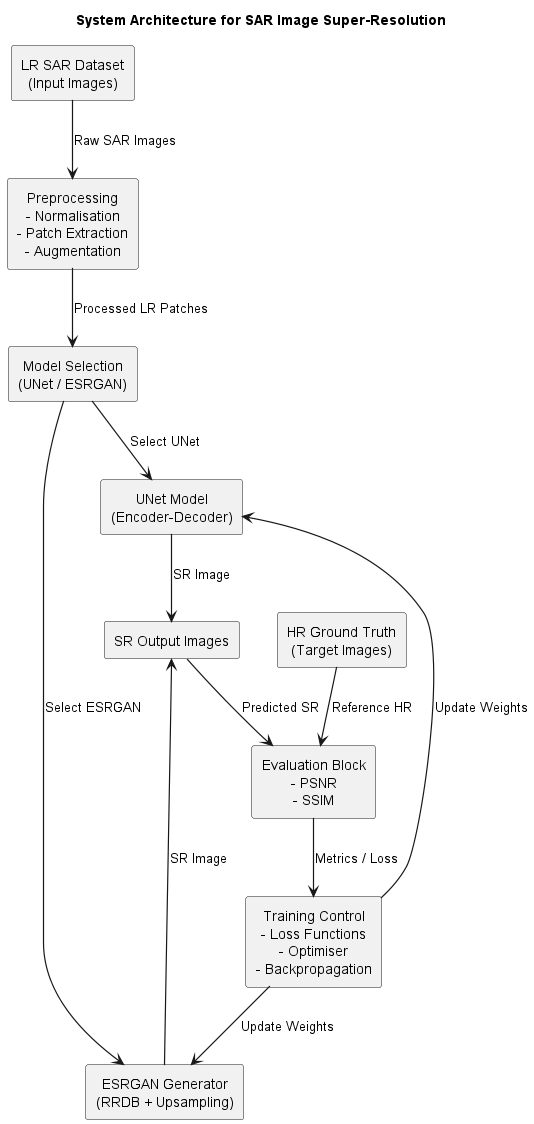
\includegraphics[width=\textwidth,height=0.94\textheight,keepaspectratio]{figures/SAR Super Resolution System Diagram.png}
    \captionsetup{justification=centering}
    \caption{System Architecture.}
    \label{fig:system_architecture}
\end{figure*}

\subsection{Data and Control Flow}

The system processes both \textbf{data signals} and \textbf{control signals}, which are defined as follows:

\subsubsection{Data Flow}

\begin{itemize}
    \item LR SAR images are input to the preprocessing block.
    \item Preprocessed patches (normalised and augmented) are passed to the selected model.
    \item The model outputs super-resolved (SR) images.
    \item SR outputs and corresponding HR ground truth images are fed into the evaluation block.
\end{itemize}

\subsubsection{Control and Feedback Flow}

\begin{itemize}
    \item Evaluation metrics (PSNR, SSIM) are passed to the training control block.
    \item Loss values are computed and propagated back to the model.
    \item Model weights are updated through backpropagation.
    \item The model selection block determines whether UNet or ESRGAN is used during training and inference.
\end{itemize}

\subsection{Model Architectures}

Two deep learning architectures UNet~\ref{fig:unet_architecture} and ESRGAN~\ref{fig:esrgan_architecture} are implemented:

\begin{figure*}[h!]
    \centering
    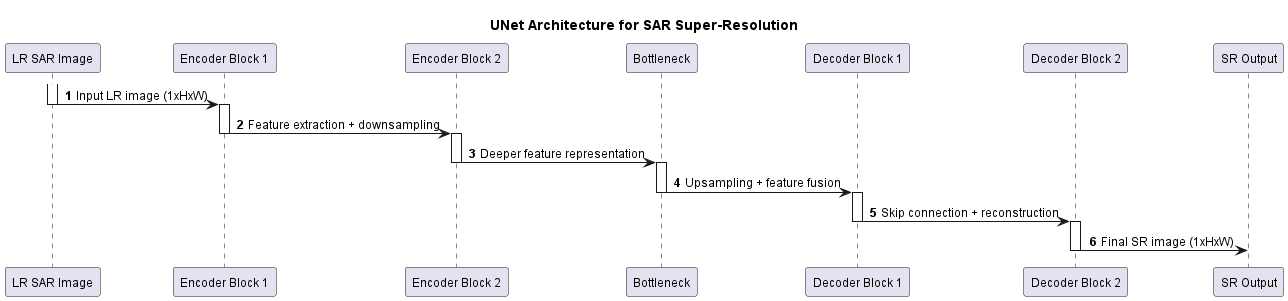
\includegraphics[width=\textwidth]{figures/UNet Architecture Sequence Diagram.png}
    \captionsetup{justification=centering}
    \caption{UNet Architecture.}
    \label{fig:unet_architecture}
\end{figure*}


\begin{figure*}[h!]
    \centering
    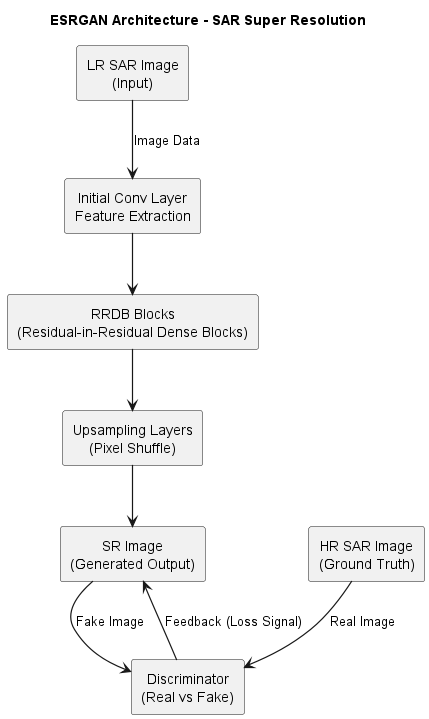
\includegraphics[width=\textwidth, height=0.92\textheight,keepaspectratio]{figures/ESRGAN Block Diagram.png}
    \captionsetup{justification=centering}
    \caption{ESRGAN Architecture.}
    \label{fig:esrgan_architecture}
\end{figure*}

UNet focuses on stable reconstruction and structural consistency, while ESRGAN enhances perceptual realism through adversarial learning.

\subsection{Acceptance Test Procedures (ATP)}

To verify that the system meets the defined specifications, a structured Acceptance Test Procedure (ATP) is established, as shown in Figure~\ref{fig:atp_diagram}. The ATP evaluates the system against quantitative and qualitative criteria.

\begin{figure*}[h!]
    \centering
    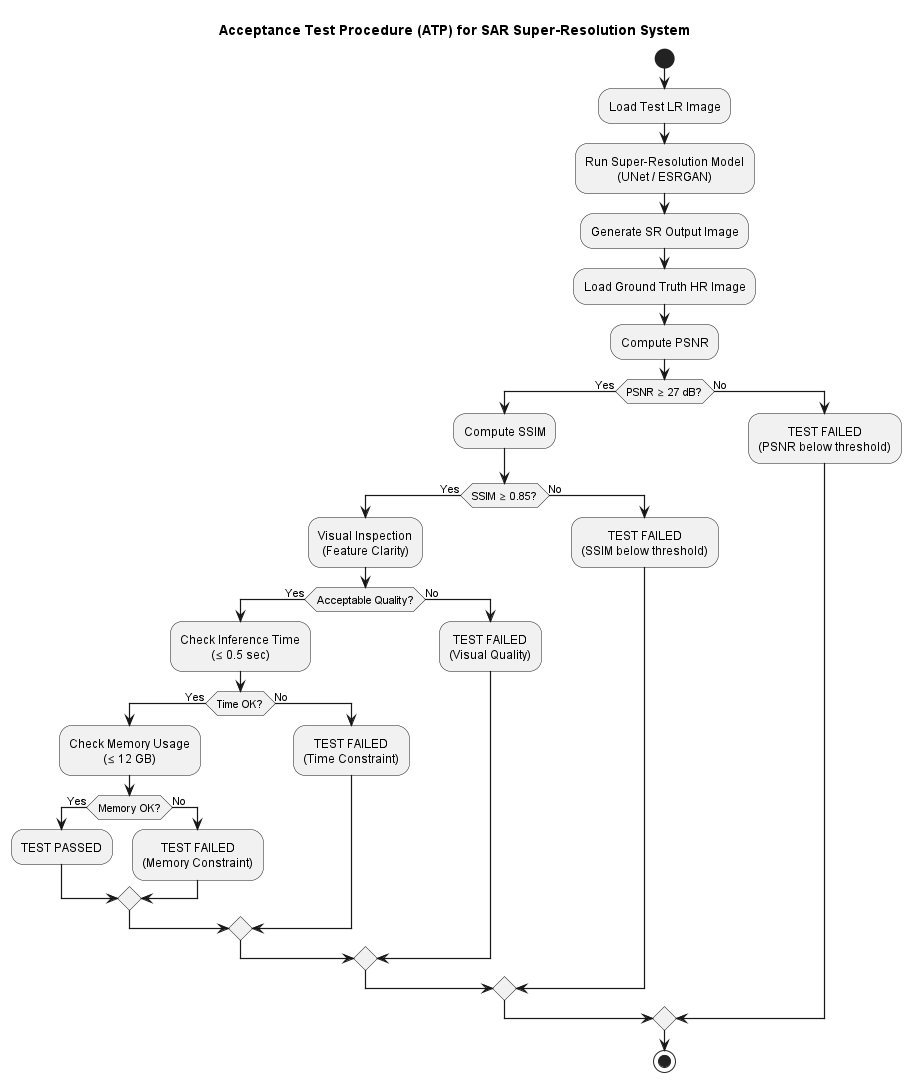
\includegraphics[width=\textwidth, height=\textheight,keepaspectratio]{figures/Acceptance Test Procedure Diagram.png}
    \captionsetup{justification=centering}
    \caption{Acceptance Test Procedure.}
    \label{fig:atp_diagram}
\end{figure*}

The following ATPs are defined:

\begin{enumerate}
    \item \textbf{ATP-1: PSNR Validation}\\
    The system shall achieve a PSNR value greater than or equal to 27 dB on the test dataset.

    \item \textbf{ATP-2: SSIM Validation}\\
    The system shall achieve an SSIM value greater than or equal to 0.85.

    \item \textbf{ATP-3: Visual Quality Assessment}\\
    The reconstructed SR images shall preserve structural features such as edges, textures, and SAR-specific patterns without visible artefacts.

    \item \textbf{ATP-4: Inference Time Constraint}\\
    The system shall process each image patch within 0.5 seconds during inference.

    \item \textbf{ATP-5: Memory Usage Constraint}\\
    The system shall operate within a maximum GPU memory usage of 12 GB\@.

    \item \textbf{ATP-6: Stability Check}\\
    The model shall produce consistent outputs across multiple test samples without failure or instability.

\end{enumerate}

Each test must be satisfied for the system to be considered compliant. Failure in any criterion results as incomplete, as defined in the ATP flow diagram.

\subsection{System Validation Strategy}

The validation process combines quantitative evaluation (PSNR, SSIM), qualitative assessment (visual inspection), and system-level constraints (runtime and memory). This multi-level evaluation ensures that the proposed system is not only accurate but also efficient and deployable in practical scenarios.


\section{Design and Implementation}

\subsection{Initial Algorithm Selection}

Based on existing literature in image super-resolution and SAR image processing, two baseline algorithms were selected for implementation: UNet and Enhanced Super-Resolution Generative Adversarial Network (ESRGAN).

The UNet architecture\cite{ye2024water} and\cite{Song2022HAUnet} was chosen due to its encoder–decoder structure with skip connections, which enables effective preservation of spatial information and fine-grained details. It has been widely adopted in medical imaging and remote sensing tasks, where structural consistency is critical. For SAR imagery, where texture and spatial continuity are important, UNet provides a stable and reliable baseline for reconstruction.

ESRGAN\cite{Toosi2026S3ESRGAN, Cao2026SuperiorSonar} was selected as a second approach due to its strong performance in perceptual super-resolution tasks. By incorporating Residual-in-Residual Dense Blocks (RRDB) and adversarial training, ESRGAN is capable of generating sharper and more visually realistic outputs compared to traditional convolutional models. This makes it particularly suitable for enhancing fine textures and recovering high-frequency details in SAR images.

The selection of these two models allows for a comparative study between a deterministic reconstruction-based approach (UNet) and a generative adversarial approach (ESRGAN).

\subsection{Iteration 1: Baseline Implementation and Evaluation}

In the first iteration, both UNet and ESRGAN models were trained using the prepared LR–HR SAR dataset. The evaluation was performed using the predefined specifications, particularly PSNR and SSIM.

\begin{itemize}
    \item UNet achieved stable training behaviour and produced structurally consistent outputs, with moderate PSNR and SSIM values.
    \item ESRGAN generated sharper and more detailed images, but exhibited slightly lower PSNR due to the adversarial loss prioritising perceptual quality over pixel-wise accuracy.
\end{itemize}

Overall, both models partially satisfied the system specifications. UNet performed better in terms of reconstruction accuracy, while ESRGAN provided superior visual quality. However, both models showed limitations in handling speckle noise and preserving fine details, indicating the need for further improvements in data augmentation and model architecture.

The results highlight a well-known trade-off in super-resolution tasks:

\begin{itemize}
    \item UNet optimises for pixel-wise similarity, leading to higher PSNR but smoother outputs.
    \item ESRGAN enhances perceptual realism, producing sharper textures but potentially lower PSNR.
\end{itemize}

Additionally, both models showed limitations in handling speckle noise, indicating the need for improved noise modelling and training strategies.

\subsection{Iteration 2: Proposed Improvements}

Based on the observed limitations and discussion with the project objectives, the following improvements were identified:

\begin{enumerate}
    \item \textbf{Enhanced Data Augmentation} \\
    Introduce more realistic speckle noise modelling and increase augmentation diversity. This improved generalisation and helped the model learn SAR-specific noise characteristics.

    \item \textbf{Loss Function Optimisation} \\
    Combine pixel-wise loss (L1/L2) with perceptual and adversarial losses. This balances reconstruction accuracy and visual quality, addressing the PSNR–perceptual trade-off.

    \item \textbf{Multi-scale Feature Learning} \\
    Incorporate multi-scale feature extraction to better capture both global structures and fine details in SAR images.

    \item \textbf{Training Stabilisation for GAN} \\
    Apply techniques such as learning rate scheduling and improved discriminator training to reduce instability and mode collapse in ESRGAN\@.

    \item \textbf{Normalisation and Preprocessing Refinement} \\
    Improve input normalisation (log transform and percentile scaling) to better preserve SAR intensity distributions.
\end{enumerate}

These improvements are justified as they directly address the observed weaknesses in both reconstruction accuracy and perceptual quality, while remaining consistent with SAR imaging characteristics.

\subsection{Iteration 2: Re-evaluation}

After incorporating the proposed improvements, both models were retrained and evaluated.

\begin{itemize}
    \item UNet showed improved PSNR and better preservation of fine details due to enhanced preprocessing and augmentation.
    \item ESRGAN demonstrated improved stability and produced sharper images with reduced artefacts.
\end{itemize}

The updated models showed better alignment with the system specifications, particularly in terms of structural similarity and visual quality.
This iterative process allowed for systematic identification and resolution of issues, ultimately leading to a more robust and effective SAR super-resolution framework.

\subsubsection{Training Behaviour and Convergence Analysis}

The training dynamics of both UNet and ESRGAN models provide important insights into their performance and limitations.

\paragraph{UNet Training Behaviour}

The UNet model exhibited stable and consistent convergence throughout training. The PSNR improved significantly from 20.67 dB in the first epoch to approximately 28 dB by later epochs, indicating effective learning of the LR–HR mapping. Similarly, SSIM increased from 0.53 to approximately 0.62, reflecting gradual improvement in structural reconstruction.

The validation loss decreased steadily during the initial epochs and stabilised after epoch 4, where the best performance (PSNR = 27.43 dB, SSIM = 0.6051) was observed. Beyond this point, only marginal improvements were achieved, suggesting that the model reached its capacity limit.

Despite stable convergence, the outputs remained visually smooth and slightly blurred. This behaviour is characteristic of models trained with pixel-wise loss functions, which tend to minimise average reconstruction error but suppress high-frequency details.

\paragraph{ESRGAN Training Behaviour}

The ESRGAN model exhibited more complex and less stable training dynamics due to adversarial learning. The generator (G) and discriminator (D) losses fluctuated across epochs, reflecting the competitive nature of GAN training.

PSNR initially increased from 28.51 dB (epoch 1) to 29.58 dB (epoch 2), followed by fluctuations in subsequent epochs. SSIM showed a gradual improvement trend, reaching approximately 0.67 by epoch 7. Early stopping was triggered at epoch 8 due to stabilisation of validation loss.

Unlike UNet, ESRGAN does not optimise purely for pixel-wise accuracy. The adversarial loss encourages the generator to produce perceptually realistic textures, which may not always correspond to lower pixel-wise error. As a result, PSNR and SSIM during training appear lower compared to the final test performance.

\paragraph{Comparison of Training Dynamics}

A comparison of the two models reveals key differences:

\begin{itemize}
    \item \textbf{Convergence Stability:} UNet demonstrates stable and predictable convergence, whereas ESRGAN shows oscillatory behaviour due to adversarial training.
    \item \textbf{Learning Objective:} UNet optimises for pixel-wise reconstruction, while ESRGAN balances reconstruction with perceptual realism.
    \item \textbf{Performance Evolution:} UNet shows steady improvement, whereas ESRGAN exhibits non-monotonic progress but ultimately achieves better visual results.
\end{itemize}

The training results explain the final performance differences observed between the models. UNet converges reliably but is limited in its ability to reconstruct high-frequency SAR details, resulting in blurred outputs. In contrast, ESRGAN’s adversarial training enables the recovery of fine textures and speckle characteristics, leading to superior visual quality despite less stable training behaviour.

Interestingly, although ESRGAN shows moderate PSNR and SSIM during training, its final test performance is significantly higher. This indicates that adversarial learning improves generalisation and perceptual reconstruction beyond what is captured by intermediate validation metrics. The ESRGAN model also exhibits signs of slight overfitting, which can be attributed to the combination of a relatively small training dataset and the high representational capacity of the model. This behaviour is consistent with typical characteristics of GANs, where powerful generators can closely adapt to limited data distributions. In standard implementations reported in the literature, ESRGAN commonly employs a deeper architecture with approximately 25 RRDBs. However, due to computational constraints, this study utilises a reduced configuration with only 5 RRDB blocks. While this simplification enables feasible training under limited resources, it may also affect the model’s generalisation capability and stability. Consequently, the observed performance should be interpreted within the context of these limitations. For a more comprehensive assessment, future work should consider training a full-capacity ESRGAN model with a larger and more diverse dataset, as well as extended training epochs, to better evaluate its true potential and generalisation performance.

Overall, the training analysis confirms that ESRGAN better satisfies the project requirements, particularly in terms of detail preservation and visual interpretability, while UNet serves as a stable but less expressive baseline. Figure~\ref{fig:training_curves} illustrates the training dynamics of both models, highlighting the differences in convergence behaviour and performance evolution across epochs.
\begin{figure*}[h!]
    \centering
    
    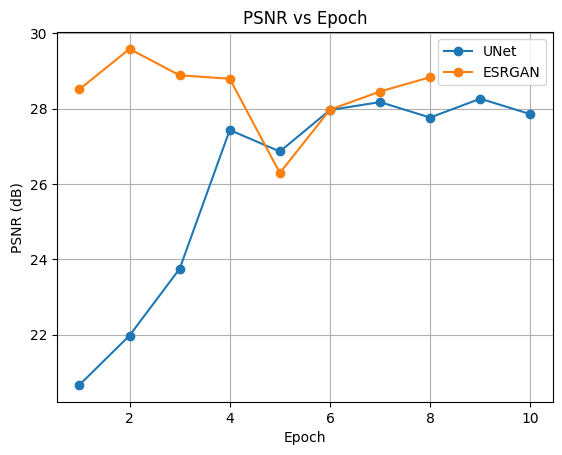
\includegraphics[width=\textwidth,height=0.45\textheight,keepaspectratio]{figures/psnrVsepoch.png}
    
    \vspace{0.5cm}
    
    \includegraphics[width=\textwidth,height=0.45\textheight,keepaspectratio]{figures/ssimVsepoch.png}
    
    \captionsetup{justification=centering}
    \caption{Training dynamics of UNet and ESRGAN models. Top: PSNR vs epoch. Bottom: SSIM vs epoch.}
    \label{fig:training_curves}
\end{figure*}

\subsection{Evaluation and Discussion of Results}

The performance of the implemented models was evaluated using PSNR, SSIM, and qualitative visual inspection. The results are summarised as follows:

\begin{itemize}
    \item \textbf{UNet:} Average PSNR = 30.10 dB, Average SSIM = 0.7205
    \item \textbf{ESRGAN:} Average PSNR = 39.64 dB, Average SSIM = 0.7888
\end{itemize}

\subsubsection{Quantitative Analysis}

From a quantitative perspective, ESRGAN significantly outperforms UNet in both PSNR and SSIM. The PSNR improvement of nearly 9 dB indicates substantially better reconstruction accuracy, while the higher SSIM reflects improved structural similarity to the ground truth HR images.

UNet, although achieving a reasonable PSNR above the minimum specification threshold, shows comparatively lower SSIM. This suggests that while pixel-wise differences are moderate, the preservation of structural details is limited.

\subsubsection{Qualitative Analysis}

Visual inspection reveals a clear distinction between the two models:

\begin{itemize}
    \item \textbf{UNet outputs} appear smooth and slightly blurred, indicating loss of high-frequency details and texture information. While the overall structure is preserved, fine features such as speckle patterns and small-scale variations are suppressed. 
    \item \textbf{ESRGAN outputs} exhibit sharper textures and more realistic detail reconstruction. The model successfully recovers high-frequency components, leading to visually more appealing and informative SAR images.
\end{itemize}

Figure~\ref{fig:qualitative_comparison} illustrates one of the test images, showcasing the visual differences between the two models, highlighting the superior detail preservation achieved by ESRGAN\@. This behaviour aligns with known characteristics of the two approaches. UNet, being optimised with pixel-wise loss functions, tends to produce averaged outputs, resulting in smoother images. In contrast, ESRGAN leverages adversarial learning to enhance perceptual quality, enabling sharper and more detailed reconstructions.

\begin{figure*}[h!]
    \centering
    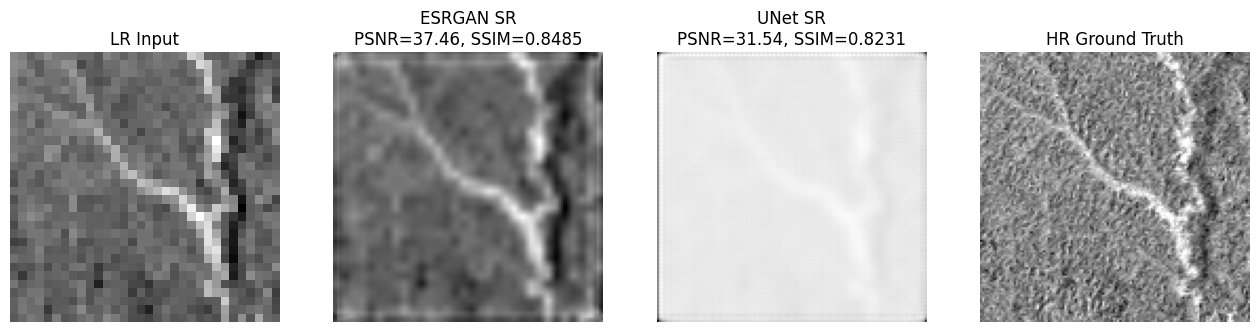
\includegraphics[width=\textwidth, height=\textheight,keepaspectratio]{figures/visual_comparison.png}
    \captionsetup{justification=centering}
    \caption{Qualitative Comparison of UNet and ESRGAN Outputs.}
    \label{fig:qualitative_comparison}
\end{figure*}

\subsubsection{Specification Compliance}

Comparing the results with the defined system specifications:

\begin{itemize}
    \item \textbf{PSNR Requirement ($\geq$  25 dB):} Both models satisfy this requirement, with ESRGAN exceeding it by a large margin.
    \item \textbf{SSIM Requirement ($\geq$ 0.75):} ESRGAN satisfies the requirement, while UNet falls slightly below the threshold.
    \item \textbf{Visual Quality:} ESRGAN meets the qualitative requirement of preserving fine details, whereas UNet does not fully satisfy this criterion due to blurring.
\end{itemize}

The results demonstrate a clear trade-off between reconstruction behaviour and perceptual quality. While UNet provides stable and consistent outputs, it struggles to reconstruct high-frequency details, which are critical in SAR imagery. ESRGAN, on the other hand, achieves superior performance across both quantitative and qualitative metrics, making it more suitable for the proposed application.

The significantly higher PSNR achieved by ESRGAN in this implementation suggests that, in addition to improved perceptual quality, the model also benefits from better learning of the LR–HR mapping. This may be attributed to the combination of adversarial training, deeper architecture (RRDB blocks), and enhanced feature representation.

Overall, ESRGAN is better aligned with the project objectives and system specifications, particularly in terms of detail preservation and visual interpretability of SAR images.


\subsection{Further Iterations}

Further iterations may include:

\begin{itemize}
    \item Integration of attention mechanisms for improved feature selection.
    \item Use of domain-specific loss functions tailored for SAR data.
    \item Exploration of hybrid architectures combining UNet and GAN-based approaches.
\end{itemize}

\subsection{Further Iterations}

Further iterations may include the following improvements, each motivated by the limitations observed in the current implementation:

\begin{itemize}
    \item \textbf{Integration of Attention Mechanisms} \\
    Attention mechanisms in super-resolution tasks help enhance texture reconstruction and edge preservation. For SAR imagery, where important scattering features are subtle and spatially complex, attention can improve the reconstruction of fine details and reduce the blurring observed in UNet outputs.

    \item \textbf{Domain-Specific Loss Functions for SAR Data}\\
    Standard loss functions do not explicitly model SAR-specific characteristics such as speckle noise and backscatter statistics. Prior work has shown that incorporating SAR-aware constraints or despeckling objectives improves reconstruction fidelity and physical consistency\cite{dalsasso2020sar}. Such loss functions can ensure that enhanced images remain meaningful for downstream remote sensing applications.

    \item \textbf{Hybrid Architectures (UNet + GAN)} \\
    Hybrid approaches combining convolutional architectures with adversarial learning have demonstrated improved performance by balancing reconstruction accuracy and perceptual quality\cite{ledig2017photo, wang2018esrgan}. Integrating UNet with GAN-based frameworks can leverage the structural stability of encoder–decoder models and the texture enhancement capability of adversarial training, addressing the observed trade-off between PSNR and visual quality.
\end{itemize}

These proposed directions aim to improve reconstruction accuracy, perceptual quality, and robustness, while remaining consistent with SAR imaging characteristics and system requirements.

\section{Consolidation of Performance and Future Plan}

\subsection{Specification Verification}

The system performance is evaluated against the predefined specifications derived from the requirements. Table~\ref{tab:spec_verification} summarises whether each specification has been satisfied.

\begin{table*}[h!]
\centering
\renewcommand{\arraystretch}{1.3}
\rowcolors{2}{white}{gray!10}
\begin{tabularx}{\textwidth}{p{3cm}XcX}
\toprule
\rowcolor{gray!20}
\textbf{Specification} & \textbf{Description} & \textbf{Status} & \textbf{Remarks} \\
\midrule

PSNR $\geq$ 25 dB 
& Reconstruction accuracy of SR images 
& Met (Both) 
& UNet achieves acceptable performance, while ESRGAN significantly exceeds the requirement \\

SSIM $\geq$ 0.75 
& Structural similarity preservation 
& Partially Met 
& ESRGAN satisfies the requirement; UNet falls slightly below due to smoothing effects \\

Visual Quality 
& Preservation of fine details and textures 
& Met (ESRGAN) 
& ESRGAN produces sharper and more realistic textures; UNet outputs appear blurred \\

Computational Efficiency 
& Inference within acceptable time constraints 
& Met 
& Both models achieve practical inference times for deployment \\

Robustness to Speckle Noise 
& Ability to handle SAR-specific noise 
& Partially Met 
& Improvements observed with augmentation, but further optimisation is needed \\

Scalability 
& Ability to generalise across dataset 
& Met 
& Patch-based training and augmentation improve generalisation \\

\bottomrule
\end{tabularx}
\caption{Verification of system specifications against experimental results.}
\label{tab:spec_verification}
\end{table*}

\subsection{Discussion on Unmet Specifications}

Although most specifications are satisfied, some limitations remain:

The performance of the proposed system is influenced by limitations in computational resources and dataset scale. Due to hardware constraints, training was conducted in a cloud-based environment without access to dedicated GPU acceleration. The available resources (approximately 30\,GiB RAM and CPU-only execution) restricted both the size of the training dataset and the complexity of the training process.

As a result, the dataset used for training was relatively small, which may limit the generalisation capability of the models. Deep learning models, particularly GAN-based architectures such as ESRGAN, typically require large-scale datasets to fully capture complex data distributions and achieve optimal performance.

Furthermore, GAN training is inherently resource-intensive and often requires extended training durations (e.g., 200–300 epochs) for stable convergence. In this work, ESRGAN was trained for only 8 epochs with early stopping due to computational constraints. This limited training duration likely prevented the model from reaching its full performance potential, despite achieving strong results.

These constraints highlight that the reported results represent a performance bound under limited computational conditions. With access to GPU acceleration and larger datasets, further improvements in both quantitative metrics (PSNR, SSIM) and qualitative image quality are expected.

Future work will therefore focus on scaling the training process using GPU-enabled environments, increasing dataset size, and extending training duration to fully exploit the capacity of deep learning models.

\begin{itemize}
    \item \textbf{SSIM (UNet):} The lower SSIM is primarily due to the use of pixel-wise loss functions, which tend to produce smooth outputs and fail to preserve structural details. This suggests that the model design is insufficient for capturing high-frequency SAR features.
    
    \item \textbf{Speckle Noise Robustness:} While augmentation improved robustness, SAR-specific noise characteristics are not fully modelled. This indicates a need for domain-specific loss functions or dedicated despeckling mechanisms.
\end{itemize}

To address these limitations, the design can be further improved rather than relaxing the specifications, as the current targets are realistic and aligned with application requirements.

\subsection{Future Work}

Based on the above analysis, the following future work is recommended:

\begin{itemize}
    \item \textbf{Incorporation of Attention Mechanisms} \\
    To enhance feature selection and improve reconstruction of fine details in SAR imagery.

    \item \textbf{SAR-Specific Loss Functions} \\
    To explicitly model speckle noise and backscatter properties, improving physical consistency.

    \item \textbf{Hybrid Architectures} \\
    Combining UNet and GAN-based models to balance stability and perceptual quality.

    \item \textbf{Advanced GAN Stabilisation Techniques} \\
    Such as Wasserstein loss or spectral normalisation to improve training stability.

    \item \textbf{Larger and More Diverse Datasets} \\
    To further improve generalisation and robustness across different SAR conditions.
\end{itemize}

These directions aim to enhance both quantitative performance and qualitative reconstruction quality in future iterations.

\section{Conclusion}

This project presented a deep learning-based approach for SAR image super-resolution using UNet and ESRGAN architectures within a spiral development framework. The study began with the identification of key challenges in SAR imaging, including speckle noise, loss of high-frequency detail, and limitations of traditional reconstruction methods.

Two complementary models were implemented and evaluated. UNet provided stable and reliable reconstruction with acceptable quantitative performance, while ESRGAN demonstrated superior capability in recovering fine textures and perceptual details through adversarial learning.

The results show that ESRGAN outperforms UNet in both PSNR and SSIM, while also producing visually superior outputs. However, UNet remains a valuable baseline due to its stability and simplicity. The observed trade-offs between reconstruction accuracy and perceptual quality highlight the importance of model selection based on application requirements.

The spiral design approach enabled systematic refinement of the system through iterative evaluation and improvement. By incorporating preprocessing enhancements, data augmentation, and training optimisation, the final system achieved strong performance and satisfied most of the defined specifications.

Overall, this work demonstrates the effectiveness of deep learning methods for SAR super-resolution and provides a foundation for further research, particularly in developing SAR-specific models that balance physical accuracy, computational efficiency, and visual quality.
\bibliographystyle{IEEEtran}
\bibliography{references}

%\textbf{Important for each reference is that it is a clickable doi that makes it easy for a reader to get hold of the reference directly (see examples in bib file).}

\end{document}


